\subsection{Diskrete Fouriertransformation (DFT)}\label{sec:dft}

Die \gls{dft} ist die zeit- und wertdiskrete Variante der Fouriertransformation, die statt von $-\infty$ bis $\infty$ über einen Vektor von N Werten, also von 0 bis N-1 läuft. 
Dies hat zur Folge, dass sich ihr Frequenzspektrum periodisch nach N Werten wiederholt.
Da es sich um eine endliche Anzahl diskreter Werte handelt, geht das Integral aus Gleichung (\ref{eq:Fouriertransformation}) in die Summe aus Gleichung (\ref{eq:dft}) über. 


Üblicherweise wird die (diskrete) Fouriertransformation genutzt, um vom Zeitbereich in den Frequenzbereich zu gelangen. In diesem Fall enthielte der Eingangsvektor 
Werte im Zeitbereich, der Ausgangsvektor Werte im Frequenzbereich.
Um von Daten im Zeitbereich sprechen zu können, müssen diese zeitlich versetzt auf den gleichen Bezugspunkt erfasst worden sein. 
Bezogen auf das Sensor-Array würde eine bestimmte Anzahl an zeitlich versetzten zeit- und wertediskretisierten Daten eines einzelnen Sensors in einem Vektor zusammengefasst 
und darauf die \gls{dft} angewandt werden, um beim Ausgangsvektor von Daten im Frequenzbereich sprechen zu können.

Statt zeitlich versetzt, werden beim Sensor-Array die Daten von mehreren Sensoren gleichzeitig erfasst. Da das Array zweidimensional ist, handelt es sich eine eine Matrix deren Sensoren verschiedene Koordinaten repräsentieren.
Aus diesem Grund muss von Orts- anstatt von
Zeitwerten gesprochen werden. Von der Transformation in das Frequenzspektrum spricht man bei Zeitwerten, da das Spektrum die Frequenzen darstellt, aus denen das Zeitsignal 
zusammengesetzt ist. Da bei der eben beschriebenen Datenerfassung Ortsdaten transformiert werden, wird von einer Transformation in den Bildbereich gesprochen. 

In dieser Arbeit werden statt Orts- und Bildbereich auch die Begriffe Eingangs- und Ausgangsvektor bzw. -matrix verwendet.

Mit der \gls{1d-dftn} wird die spaltenweise DFT einer Matrix bezeichnet, in der Regel ist sie der erste Schritt der Berechnung der \gls{2d-dft}. 
Die Größe der Eingangsmatrix gibt die Größe der Twiddlefaktormatrix vor, beide müssen identisch und
quadratisch sein. In dieser Arbeit wird die \gls{dft} einer Matrix der Größe $N$x$N$ auch $N$x$N$-\gls{dft} genannt.


\subsection{Summen- und Matrizenschreibweise der DFT}\label{sec:SummenMatrizenDFT}
\subsubsection{1D-DFT}
Die \gls{dft} findet Anwendung, um vom Zeit- bzw. Ortsbereich in den Frequenz- bzw. Bildbereich zu gelangen.
\begin{equation}\label{eq:dft}
 X^* \left[ m \right] = \frac{1}{N} \cdot \sum^{N-1}_{n=0} x[n] \cdot e^{-\frac{j 2 \pi m n}{N}}
\end{equation}


In Gleichung (\ref{eq:dft}) ist die Verwendung von Eingangsvektor $x[n]$ und Ausgangsvektor $X[n]$ zu sehen. Eine spaltenweise Multiplikationen einer Matrix
ist auch denkbar und ist darüber hinaus Grundlage für die \gls{2d-dft}.
Gleichung (\ref{eq:1D-DFT_MatrixMult}) zeigt die Summenformel aus (\ref{eq:dft}), umgeschrieben zu einer Matrixmultiplikation.

Mit Gleichung (\ref{eq:Twiddlefaktorenberechnung}) werden alle Twiddlefaktoren in Matrixform berechnet, wobei $n$ der Index des zu berechnenden Elements des 
Vektors im Zeitbereich und $m$ das Äquivalent im Frequenzbereich ist.

\begin{equation}\label{eq:Twiddlefaktorenberechnung}
W = \sum^{N-1 }_{m=0} \sum^{N-1 }_{n=0} e^{-\frac{j 2 \pi m n}{N}}
\end{equation}
Bei genauer Betrachtung fällt auf, dass sie identisch mit ihrer Transponierten ist.


Somit gilt:

\begin{equation}\label{eq:1D-DFT_MatrixMult}
X^* = W \cdot x
\end{equation}




Anhand der Summen die jeweils von 0 bis N-1 laufen, lässt sich die Anzahl der benötigten komplexen Multiplikationen $m_{DFT}$ einer DFT errechnen. Siehe auch Gleichung 
(\ref{eq:DFT_komplexMult}).

\begin{equation}\label{eq:DFT_komplexMult}
 m_{DFT} = N^2
\end{equation}


\subsubsection{2D-DFT}\label{sec:2d-dft}
Die \gls{2d-dft} wird in der Bildverarbeitung verwendet, um vom Orts- in den Fourierraum zu gelagen. Da es sich nicht um eine Abhängigkeit 
der Zeit handelt, werden andere Indizes verwendet.
\begin{align}
\begin{split}
X[u,v] 	&= \frac{1}{N} \sum^{N-1}_{n=0} X^* \left[ m \right] \cdot e^{-\frac{j 2 \pi m n}{N}}\\
	&= \frac{1}{MN} \sum^{M-1}_{m=0} \left( \sum^{N-1}_{n=0} f(m,n) \cdot e^{-\frac{j 2 \pi m n}{N}} \right) \cdot e^{-\frac{j 2 \pi m n}{M}}
\end{split}
\end{align}

Auch hier lässt sich die Berechnung in Matrizenschreibweise darstellen:

\begin{align}
\begin{split}\label{eq:2D-DFT_MatrixMult}
 X &= W \cdot x \cdot W \\
                    &= X^* \cdot W
\end{split}
\end{align}

Die Gleichungen (\ref{eq:1D-DFT_MatrixMult}) und (\ref{eq:2D-DFT_MatrixMult}) sind inn dieser Arbeit wesentlicher Bestandteil der Umsetzung der 2D-DFT.


Die 2D-DFT kann als ``doppelte'' Matrixmultiplikation geschrieben werden (Gleichung (\ref{eq:2D-DFT_MatrixMult})).
Zuerst wird die 1D-DFT berechnet und die Matrix $X^*$ wird anschließend mit der Twiddlefaktor-Matrix $W$ 
multipliziert. Man könnte es auch als zweite 1D-DFT betrachten, bei der Twiddlefaktor-Matrix und Eingangsmatrix vertauscht sind.
Veranschaulicht wird dies in den Abbildungen \ref{pic:1D-DFT_als_Matrixmultiplikation} und \ref{pic:2D-DFT_als_Matrixmultiplikation}.



\begin{figure}[ht!]
\centering
 \begingroup
 \renewcommand*{\arraystretch}{1.1} % Zeilenabstand
 \renewcommand*{\arraycolsep}{0.0pt} % Spaltenabstand
 \[
  \stackrel{\mbox{$W$}}{
   \begin{bmatrix}
    \myBlackBox 	& \myBlackBox 		& \myBlackBox 		& \myBlackBox \\
    \myLightgrayBox 	& \myLightgrayBox 	& \myLightgrayBox 	& \myLightgrayBox \\
    \myLightgrayBox 	& \myLightgrayBox	& \myLightgrayBox	& \myLightgrayBox \\
    \myLightgrayBox 	& \myLightgrayBox 	& \myLightgrayBox 	& \myLightgrayBox 
   \end{bmatrix}
  }
  \quad \cdot \quad
 \renewcommand*{\arraystretch}{0.0} % Zeilenabstand
 \renewcommand*{\arraycolsep}{0.8pt} % Spaltenabstand
  \stackrel{\mbox{$x$}}{
   \begin{bmatrix}
    \myBlackBoxHigh 	& \myBlackBoxHigh 	& \myBlackBoxHigh 	& \myBlackBoxHigh \\
    \myBlackBoxHigh 	& \myBlackBoxHigh 	& \myBlackBoxHigh 	& \myBlackBoxHigh \\
    \myBlackBoxHigh 	& \myBlackBoxHigh 	& \myBlackBoxHigh 	& \myBlackBoxHigh \\
    \myBlackBoxHigh 	& \myBlackBoxHigh 	& \myBlackBoxHigh 	& \myBlackBoxHigh 
   \end{bmatrix}
  }
 \quad = \quad
\renewcommand*{\arraystretch}{1.1} % Zeilenabstand
\renewcommand*{\arraycolsep}{0.8pt} % Spaltenabstand 
  \stackrel{\mbox{$X^*$}}{
   \begin{bmatrix}
    \myBlackBox 	& \myBlackBox 		& \myBlackBox 		& \myBlackBox \\
    \myLightgrayBox 	& \myLightgrayBox 	& \myLightgrayBox 	& \myLightgrayBox \\
    \myLightgrayBox 	& \myLightgrayBox 	& \myLightgrayBox 	& \myLightgrayBox \\
    \myLightgrayBox 	& \myLightgrayBox 	& \myLightgrayBox 	& \myLightgrayBox 
   \end{bmatrix}
  }
\]
 \endgroup
\caption{1D-DFT als Matrixmultiplikation.}
\label{pic:1D-DFT_als_Matrixmultiplikation}
\end{figure}




% 
% \begin{figure}[ht!]
% \centering 
% \begin{minipage}{0.2\textwidth}
%  \begingroup
%  \renewcommand*{\arraystretch}{1.1} % Zeilenabstand
%  \renewcommand*{\arraycolsep}{0.0pt} % Spaltenabstand
% 
%  \[
%   \stackrel{\mbox{$X^*$}}{
%    \begin{bmatrix}
%     \myBlackBox 	& \myBlackBox 		& \myBlackBox 		& \myBlackBox \\
%     \myLightgrayBox 	& \myLightgrayBox 	& \myLightgrayBox 	& \myLightgrayBox \\
%     \myLightgrayBox 	& \myLightgrayBox	& \myLightgrayBox	& \myLightgrayBox \\
%     \myLightgrayBox 	& \myLightgrayBox 	& \myLightgrayBox 	& \myLightgrayBox 
%    \end{bmatrix}
%   }
%  \]
%  \endgroup
% \end{minipage}
% \begin{minipage}{0.05\textwidth}
%  \[
%   \cdot
%  \]
% \end{minipage}
% \begin{minipage}{0.2\textwidth}
%  \begingroup
%  \renewcommand*{\arraystretch}{0.0} % Zeilenabstand
%  \renewcommand*{\arraycolsep}{0.8pt} % Spaltenabstand
% 
%  \[
%   \stackrel{\mbox{$W$}}{
%    \begin{bmatrix}
%     \myBlackBoxHigh 	& \myBlackBoxHigh 	& \myBlackBoxHigh 	& \myBlackBoxHigh \\
%     \myBlackBoxHigh 	& \myBlackBoxHigh 	& \myBlackBoxHigh 	& \myBlackBoxHigh \\
%     \myBlackBoxHigh 	& \myBlackBoxHigh 	& \myBlackBoxHigh 	& \myBlackBoxHigh \\
%     \myBlackBoxHigh 	& \myBlackBoxHigh 	& \myBlackBoxHigh 	& \myBlackBoxHigh 
%    \end{bmatrix}
%   }
%  \]
%  \endgroup
% \end{minipage}
% \begin{minipage}{0.05\textwidth}
%  \[
%   =
%  \]
% \end{minipage}
% \begin{minipage}{0.3\textwidth}
% \begingroup
% \renewcommand*{\arraystretch}{1.1} % Zeilenabstand
% \renewcommand*{\arraycolsep}{0.8pt} % Spaltenabstand
% \[
%   \stackrel{\mbox{$X$}}{
%    \begin{bmatrix}
%     \myBlackBox 	& \myBlackBox 		& \myBlackBox 		& \myBlackBox \\
%     \myLightgrayBox 	& \myLightgrayBox 	& \myLightgrayBox 	& \myLightgrayBox \\
%     \myLightgrayBox 	& \myLightgrayBox 	& \myLightgrayBox 	& \myLightgrayBox \\
%     \myLightgrayBox 	& \myLightgrayBox 	& \myLightgrayBox 	& \myLightgrayBox 
%    \end{bmatrix}
%   }
%  \]
%  \endgroup
% \end{minipage}
% \caption{2D-DFT als Matrixmultiplikation}
% \label{pic:2D-DFT_als_Matrixmultiplikation}
% \end{figure}


\begin{figure}[ht!]
\centering 
 \begingroup
 \renewcommand*{\arraystretch}{1.1} % Zeilenabstand
 \renewcommand*{\arraycolsep}{0.0pt} % Spaltenabstand
 \[
  \stackrel{\mbox{$X^*$}}{
   \begin{bmatrix}
    \myBlackBox 	& \myBlackBox 		& \myBlackBox 		& \myBlackBox \\
    \myLightgrayBox 	& \myLightgrayBox 	& \myLightgrayBox 	& \myLightgrayBox \\
    \myLightgrayBox 	& \myLightgrayBox	& \myLightgrayBox	& \myLightgrayBox \\
    \myLightgrayBox 	& \myLightgrayBox 	& \myLightgrayBox 	& \myLightgrayBox 
   \end{bmatrix}
  }
  \quad \cdot \quad
 \renewcommand*{\arraystretch}{0.0} % Zeilenabstand
 \renewcommand*{\arraycolsep}{0.8pt} % Spaltenabstand
  \stackrel{\mbox{$W$}}{
   \begin{bmatrix}
    \myBlackBoxHigh 	& \myBlackBoxHigh 	& \myBlackBoxHigh 	& \myBlackBoxHigh \\
    \myBlackBoxHigh 	& \myBlackBoxHigh 	& \myBlackBoxHigh 	& \myBlackBoxHigh \\
    \myBlackBoxHigh 	& \myBlackBoxHigh 	& \myBlackBoxHigh 	& \myBlackBoxHigh \\
    \myBlackBoxHigh 	& \myBlackBoxHigh 	& \myBlackBoxHigh 	& \myBlackBoxHigh 
   \end{bmatrix}
  }
  \quad = \quad
\renewcommand*{\arraystretch}{1.1} % Zeilenabstand
\renewcommand*{\arraycolsep}{0.8pt} % Spaltenabstand
  \stackrel{\mbox{$X$}}{
   \begin{bmatrix}
    \myBlackBox 	& \myBlackBox 		& \myBlackBox 		& \myBlackBox \\
    \myLightgrayBox 	& \myLightgrayBox 	& \myLightgrayBox 	& \myLightgrayBox \\
    \myLightgrayBox 	& \myLightgrayBox 	& \myLightgrayBox 	& \myLightgrayBox \\
    \myLightgrayBox 	& \myLightgrayBox 	& \myLightgrayBox 	& \myLightgrayBox 
   \end{bmatrix}
  }
 \]
 \endgroup
\caption{2D-DFT als Matrixmultiplikation.}
\label{pic:2D-DFT_als_Matrixmultiplikation}
\end{figure}




\subsection{2D-DFT mit reellen Eingangswerten}\label{sec:rein_reelle_dft}
Bei der oben beschriebenen Berechnung können die Eingangssignale auch komplex sein. Da das Ausgangssignal der \gls{1d-dft} unabhängig von den Eingangssignalen 
komplex ist, kann es direkt als Eingangssignal für die komplexe \gls{2d-dft} genutzt werden. 

Das komplexe Ausgangssignal der \gls{1d-dft} kann auch als zwei von einander unabhängige rein reelle Eingangssignale der 2D-DFTs betrachtet und später 
wieder zusammenzusetzen werden. Gleiches gilt für ein komplexes Eingangssignal, welches in zwei von einander unabhängigen DFTs transformiert werden kann.
Da bei dieser Umsetzung kein Imaginärteil in die Berechnung der Ergebnisse einfließt, hat sie den Vorteil, dass aus Symmetriegründen die Hälfte der Multiplikationen 
eingespart werden können. Es ist erforderlich, dass der Imaginärteil der gespiegelten Ergebnisse negiert wird. Abbildung \ref{pic:reelleMatMultRedundanz} zeigt die 
redundanten Werte der DFT. Demnach müssen bei der 8x8-DFT statt 16 nur 8 Multiplikationen mit reellem Multiplikand und komplexem Multiplkator erfolgen.
%Dieses Verfahren lässt sich auch für komplexe Eingangssignale, deren Real- und Imaginärteil separat voneinander mit der DFT transformiert werden, anwenden.
Anschließend müssen die Ergebnisse, wie in Abb. \ref{pic:reelleDFT} zu sehen, zusammengesetzt werden. 
%Wie dies geschieht, ist der Abbildung \ref{pic:reelleDFT} zu entnehmen.
Die Abbildung stellt die schematische Berechnung der \gls{2d-dft} eines reellen Eingangssignals dar. 
Um die \gls{2d-dft} eines komplexen Eingangssignals zu berechnen, müssen bei dieser Methode zwei identische Recheneinheit vorhanden, wenn Real- und Imaginärteil parallel berechnet werden sollen.
Andernfalls müssen sie zeitlich versetzt berechnet und  Zwischenergebnisse gespeichert werden. 
Die Ergebnisse beider 2D-DFTs müssen identisch zusammengefasst werden, wie es zum Abschluss der einzelnen 2D-DFTs geschehen muss.

\begin{figure}[htbp]
 \centering
   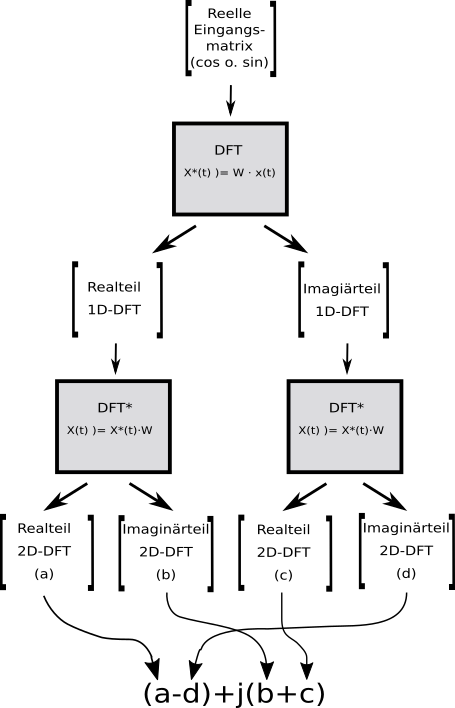
\includegraphics[width=0.6\textwidth]{img/reelleMatMult.png}
 \caption{Veranschaulichung der Berechnung der DFT mit reellen Eingangswerten.}
 \label{pic:reelleDFT}
\end{figure}


\begin{figure}[htbp]
 \centering
  \begin{subfigure}{.5\textwidth}
  \centering
   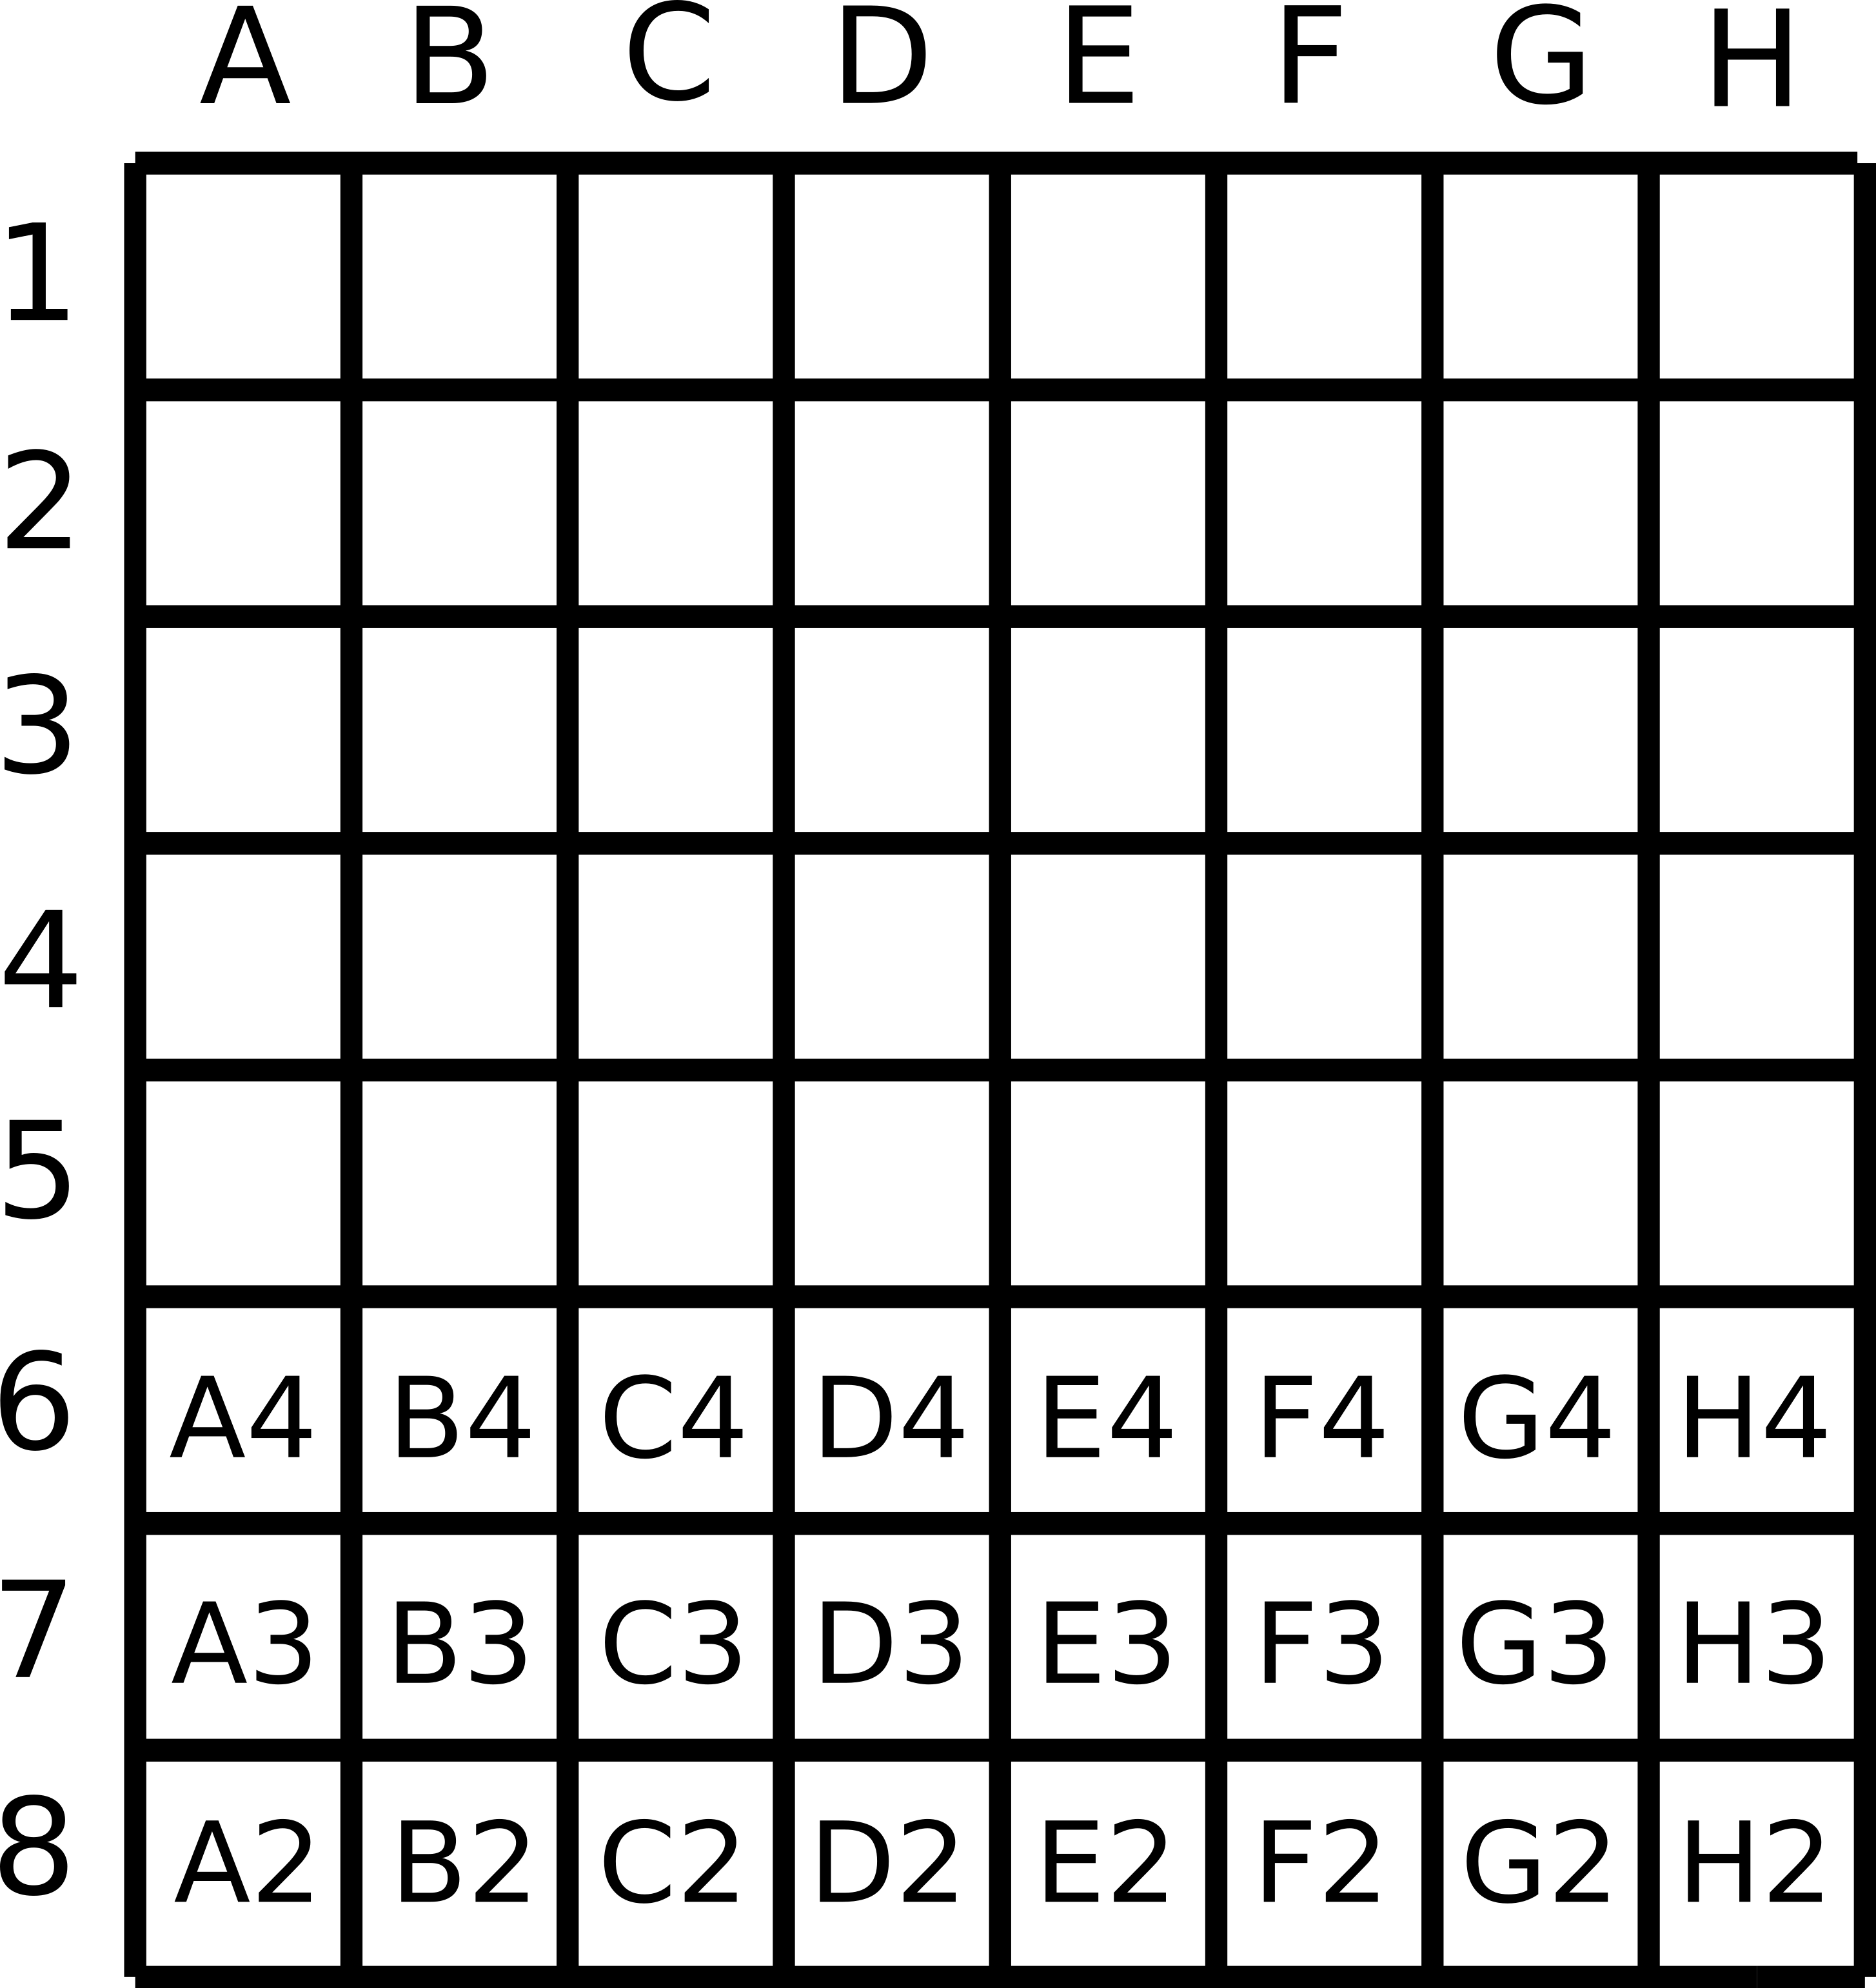
\includegraphics[width=0.8\textwidth]{img/reelleMatMultRedundanzRealteil.png}
   \caption{Realteil}
  \end{subfigure}%
  \begin{subfigure}{.5\textwidth} 
   \centering
   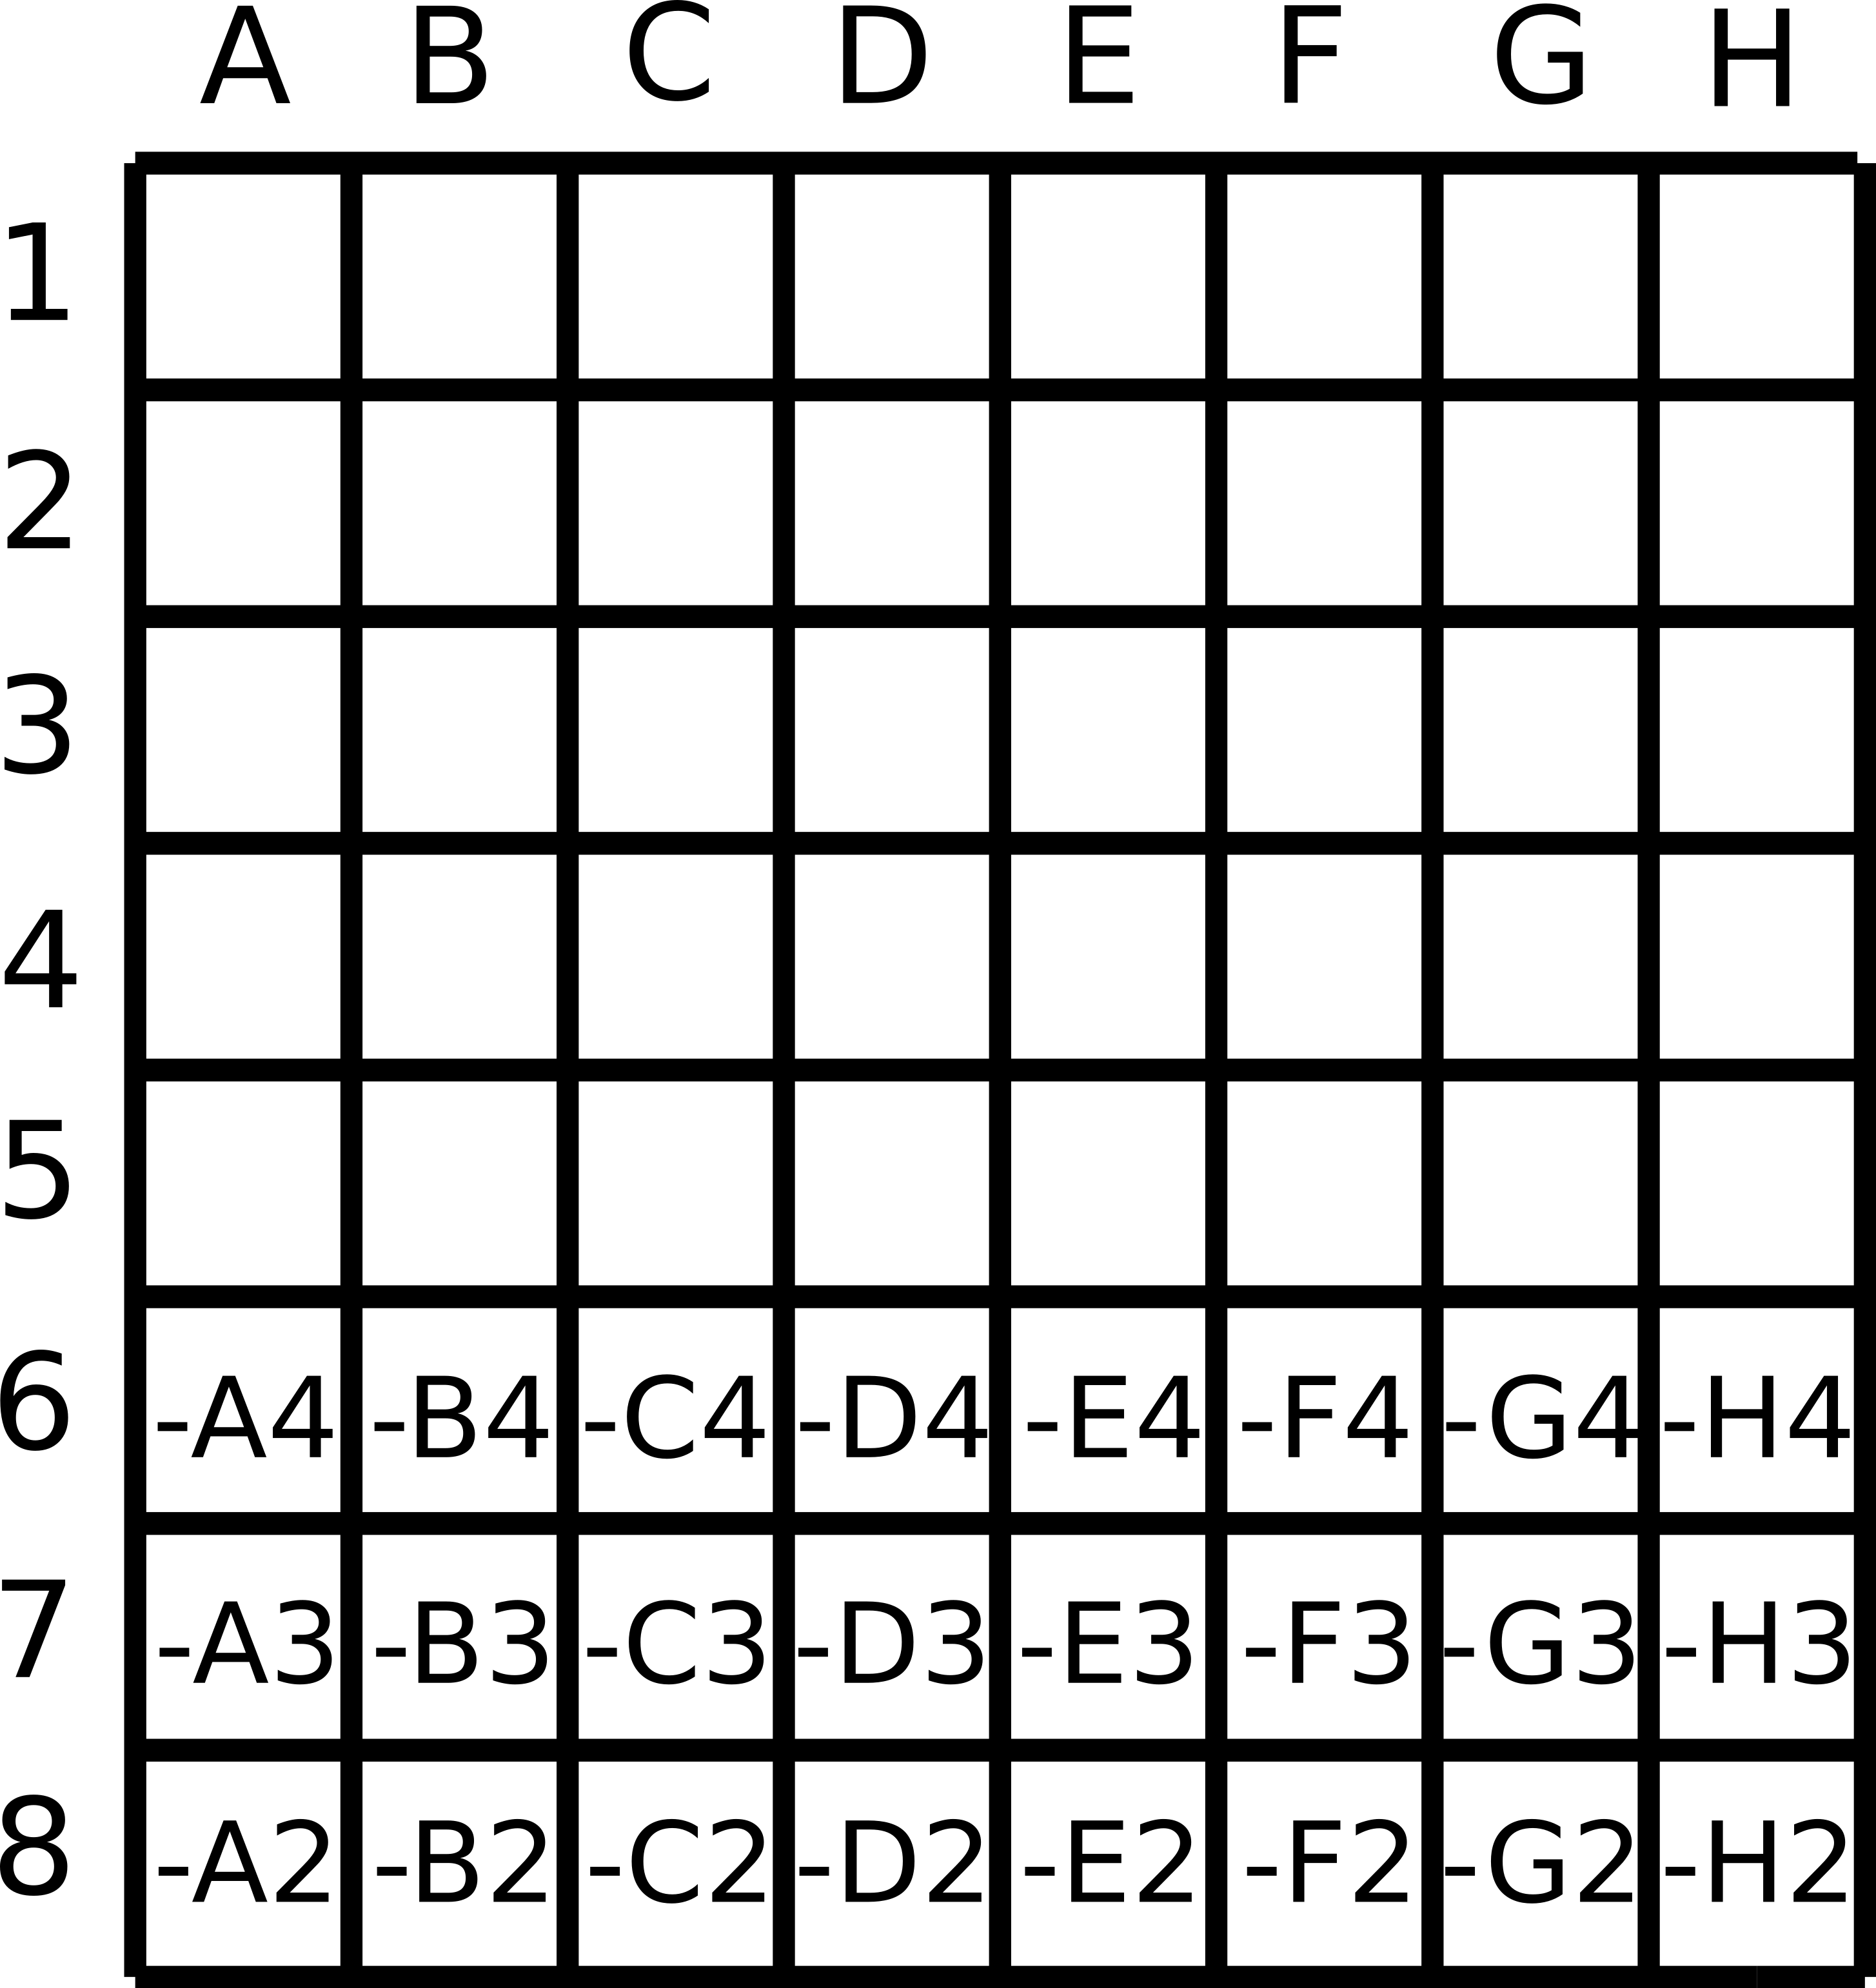
\includegraphics[width=0.8\textwidth]{img/reelleMatMultRedundanzImagteil.png}
   \caption{negierter Imaginärteil}
  \end{subfigure}
  \caption{Redundante Werte der spaltenweisen DFT einer 8x8-Matrix. Der Imaginärteil der redundanten Werte hat denselben Betrag mit negiertem Vorzeichen.}
 \label{pic:reelleMatMultRedundanz}
\end{figure}




Da die gegebenen Eingangssignale aus einer Sinus- und einer Kosinuskomponente bestehen und es sich auf diese Weise als ein komplexes Signal auffassen lässt, kann die 
komplexe Berechnung sowohl bei der 1D-DFT als auch bei der 2D-DFT genutzt werden. 
Da hierdurch in beiden Fällen eine vollständige Auslastung einer komplexen Berechnung gegeben ist und wie bereits erwähnt, bei der reellen Berechnung zusätzlicher Speicher 
erforderlich wäre, wird dieses Verfahren angewandt.



